\documentclass[12pt,a4paper]{scrartcl}\usepackage[]{graphicx}\usepackage[]{color}
%% maxwidth is the original width if it is less than linewidth
%% otherwise use linewidth (to make sure the graphics do not exceed the margin)
\makeatletter
\def\maxwidth{ %
  \ifdim\Gin@nat@width>\linewidth
    \linewidth
  \else
    \Gin@nat@width
  \fi
}
\makeatother

\definecolor{fgcolor}{rgb}{0.345, 0.345, 0.345}
\newcommand{\hlnum}[1]{\textcolor[rgb]{0.686,0.059,0.569}{#1}}%
\newcommand{\hlstr}[1]{\textcolor[rgb]{0.192,0.494,0.8}{#1}}%
\newcommand{\hlcom}[1]{\textcolor[rgb]{0.678,0.584,0.686}{\textit{#1}}}%
\newcommand{\hlopt}[1]{\textcolor[rgb]{0,0,0}{#1}}%
\newcommand{\hlstd}[1]{\textcolor[rgb]{0.345,0.345,0.345}{#1}}%
\newcommand{\hlkwa}[1]{\textcolor[rgb]{0.161,0.373,0.58}{\textbf{#1}}}%
\newcommand{\hlkwb}[1]{\textcolor[rgb]{0.69,0.353,0.396}{#1}}%
\newcommand{\hlkwc}[1]{\textcolor[rgb]{0.333,0.667,0.333}{#1}}%
\newcommand{\hlkwd}[1]{\textcolor[rgb]{0.737,0.353,0.396}{\textbf{#1}}}%
\let\hlipl\hlkwb

\usepackage{framed}
\makeatletter
\newenvironment{kframe}{%
 \def\at@end@of@kframe{}%
 \ifinner\ifhmode%
  \def\at@end@of@kframe{\end{minipage}}%
  \begin{minipage}{\columnwidth}%
 \fi\fi%
 \def\FrameCommand##1{\hskip\@totalleftmargin \hskip-\fboxsep
 \colorbox{shadecolor}{##1}\hskip-\fboxsep
     % There is no \\@totalrightmargin, so:
     \hskip-\linewidth \hskip-\@totalleftmargin \hskip\columnwidth}%
 \MakeFramed {\advance\hsize-\width
   \@totalleftmargin\z@ \linewidth\hsize
   \@setminipage}}%
 {\par\unskip\endMakeFramed%
 \at@end@of@kframe}
\makeatother

\definecolor{shadecolor}{rgb}{.97, .97, .97}
\definecolor{messagecolor}{rgb}{0, 0, 0}
\definecolor{warningcolor}{rgb}{1, 0, 1}
\definecolor{errorcolor}{rgb}{1, 0, 0}
\newenvironment{knitrout}{}{} % an empty environment to be redefined in TeX

\usepackage{alltt}
\usepackage[utf8]{inputenc}
\usepackage{amsmath}
\usepackage{graphicx}
\usepackage{tikz}
%\usepackage{silence}
\usepackage{mdframed}
%\WarningFilter{mdframed}{You got a bad break}
\usepackage[colorinlistoftodos]{todonotes}
\usepackage{listings}
\usepackage{color}
\colorlet{exampcol}{blue!10}
\usepackage{multicol}
\usepackage{booktabs}

\usepackage{exercise}

\usepackage[autostyle, english = american]{csquotes}
\MakeOuterQuote{"}

\usepackage{hyperref}
\hypersetup{
    colorlinks,
    citecolor=black,
    filecolor=black,
    linkcolor=blue,
    urlcolor=black
}

\title{Exercises for statistical inference and stuff}
\date{\today}
\author{Timoth\'ee Bonnet}
\IfFileExists{upquote.sty}{\usepackage{upquote}}{}
\begin{document}


\maketitle

\tableofcontents
\ListOfExerciseInToc
\ExerciseLevelInToc{subsubsection}

\clearpage

\section{Understanding error structure}

\subsection{Broken experiments}

\begin{Exercise}[difficulty=1, title={A significant result?}]
We carry out a vaccine challenge experiment. There are three experimental groups (saline control / low vaccine dose / high vaccine dose), with 6 mice in each group. For each group all mice are housed together in the same cage (so there are three cages). All mice are challenged with \emph{Shigella}, their symptom intensity is scored on day 8. A one-way ANOVA identifies an effect of the treatment, and pair-wise Bonferroni tests show the low-dose to be statistically significant different from the two other groups:

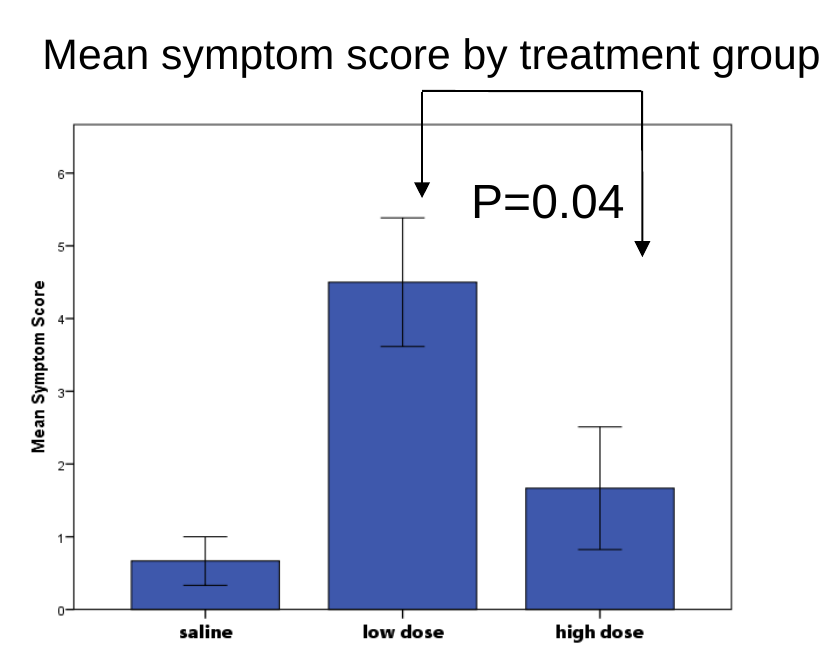
\includegraphics[width=0.4\textwidth]{Figures/message1}

\textbf{What is suspicious in the result? What part of the design may explain the result? How to improve the design (there are at least two different ways)?}
\end{Exercise}


\begin{Exercise}[difficulty=1, title={A better experimental design}]
We study how a membrane protein intakes external molecules in frog eggs. The target molecules are radioactively labelled so we can measure intake. We created five mutant lines to test what part of the protein controls intake. We propose to measure six tubes of ten eggs every week. Each week we will test a different genotype (i.e., the control or one of the five mutants):

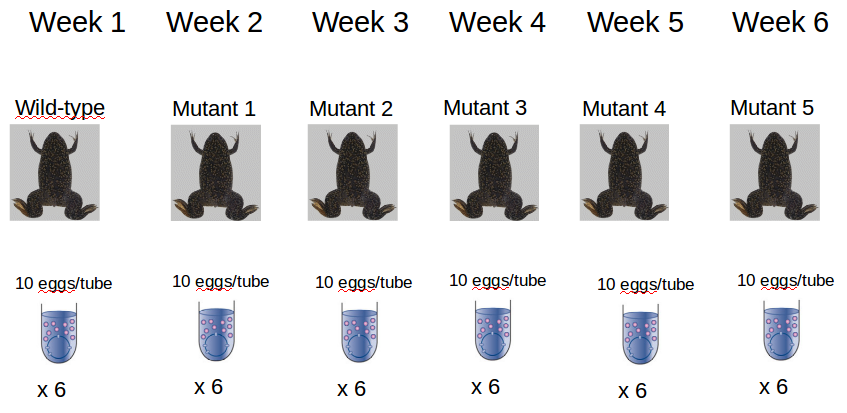
\includegraphics[width=0.8\textwidth]{Figures/expdes2}

\textbf{How much information about mutants can we extract from this experiment? How to improve the design?}

\end{Exercise}


\subsection{Broken models?}

Let's look at models with data from the an experiment similar to the mice example.
\begin{Exercise}[difficulty=1, title={lm vs. lmer vs. lm+}]

Load the dataset "challenge2.csv", and test the effect of the vaccine treatment ("Group") on the immune response ("Percent.loss"). 
First fit a fixed-effect only linear model and/or an anova. Is there a clear effect of treatment?\\
Now add a random effect for Cage (e.g., using the package lme4), what happens to the effect of treatment?\\
Finally, fit Cage and Group as fixed effects in a simple linear model and/or anova. What happens, why?\\
Which of the three models should you trust or not?

\end{Exercise}




\subsection{Experimental design}


\begin{Exercise}[difficulty=1]
\textbf{Use a for loop and an if-else statement to do that.}
\end{Exercise}


\section{Interpreting simple mixed models}

\section{Flexible variance structures}



\end{document}
